\scanpage{48}
\mspage{\handwritten{16}}
\uline{Then, for every quasi-coherent sub-$\handwritten{\mathcal{O}}_S$-Module $\handwritten{\mathcal{F}}$ of $\handwritten{\mathcal{E}}$ there exists a smallest quasi-coherent sub-$\handwritten{\mathcal{O}}_S$-Mo-\linebreak dule $\handwritten{\widetilde{\mathcal{F}}}$ of $\handwritten{\mathcal{E}}$ containing $\handwritten{\mathcal{F}}$ which is stable under $\handwritten{\rho}$.}\inserted{\figure{\handwritten{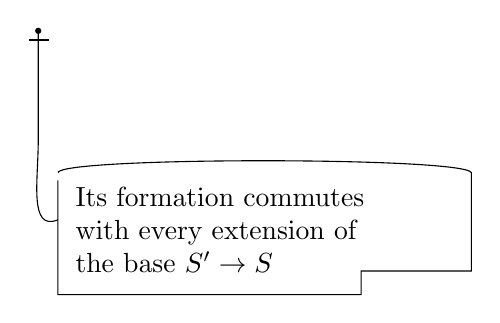
\begin{tikzpicture}[x=1cm,y=1cm]
\draw (.25,.1) .. controls (-.12,-.05) and (0,.6) .. (0,1.1) -- (0,2.5);
\fill (0,2.5) circle (.04);\draw[line width=.8pt] (-.12,2.38) -- (.14,2.38);
\draw (.25,.7) .. controls (.3,.9) and (5.4,.9) .. (5.5,.7) -- (5.5,-.55) -- (4.1,-.55) -- (4.1,-.85) -- (.25,-.85) -- (.25,.60);
\node[align=left,anchor=west] at (.35,-.03) {Its formation commutes\\with every extension of\\the base $S'\to S$};
\end{tikzpicture}}}}\uline{When $\handwritten{\mathcal{F}}$ is of \deleted{\illegible{1}} finite type, the same holds for $\handwritten{\mathcal{F}}$.}

One easily reduces\inserted{\handwritten{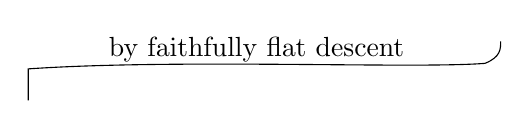
\begin{tikzpicture}[x=1cm,y=1cm,baseline=(n.base)]\node (n) at (0,0) {by faithfully flat descent};\draw (-2.9,-.65)--(-2.9,-.25) .. controls (-1,-.12) and (2,-.25) .. (2.9,-.18) .. controls (3.1,-.1) and (3.1,0) .. (3.1,.1);\end{tikzpicture}}} to the case where $\handwritten{\unsure{\mathcal{A}|a}}$ is a free $\handwritten{\mathcal{O}}_S$-Module, in which case the proposition is a consequence of lemma 11.8.

\figure{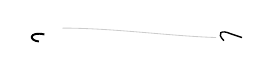
\begin{tikzpicture}[x=1cm,y=1cm]\draw[line width=.7pt] (.12,.04) .. controls (-.08,.08) and (-.08,-.04) .. (.05,-.05);\draw[gray!40,line width=.3pt] (.35,.12) .. controls (1,.12) and (1.7,.02) .. (2.3,0);\draw[line width=.5pt] (2.4,-.04) .. controls (2.3,.06) and (2.37,.1) .. (2.48,.05)--(2.63,0);\end{tikzpicture}}
\uline{Corollary 11.10.- \deleted{Let}\inserted{Let} $S$ be a \deleted{affine}\inserted{\handwritten{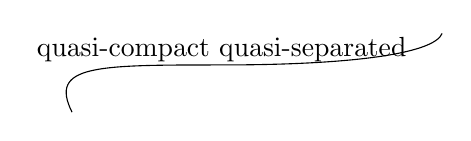
\begin{tikzpicture}[x=1cm,y=1cm,baseline=(n.base)]\node (n) at (0,0) {quasi-compact quasi-separated};\draw (-1.9,-.8) .. controls (-2.2,-.2) and (-1.6,-.2) .. (0,-.2) .. controls (1.7,-.2) and (2.7,-.05) .. (2.8,.2);\end{tikzpicture}}} \deleted{pre}scheme, $G$ an $S$-group quasi-separated\inserted{\handwritten{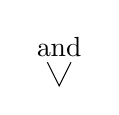
\begin{tikzpicture}[x=1cm,y=1cm,baseline=(n.base)]\node (n) at (0,0) {and};\draw (-.15,-.2)--(0,-.5)--(.15,-.2);\end{tikzpicture}}}quasi-compact over $S$ , such that $\handwritten{\mathcal{A}}(G)$ becomes \deleted{\unsure{free}} locally free after a faithfully flat quasi-com-\linebreak pact extension of the base,$S$, and let $\handwritten{\mathcal{E}}$ be a quasi-coherent $\handwritten{\mathcal{O}}_S$-Module. We assume either that $G$ is affine over $S$\deleted{\unsure{.}}\handwritten{,}or that $G$ and $\handwritten{\mathcal{E}}$ are flat over $S$,\inserted{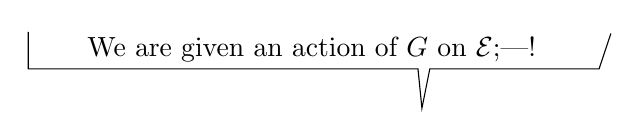
\begin{tikzpicture}[x=1cm,y=1cm,baseline=(n.base)]\node (n) at (0,0) {\uline{We are given an action of $G$ on $\handwritten{\mathcal{E}}$\handwritten{\unsure{;|!}}}};\draw (-3.6,.22)--(-3.6,-.25)--(1.35,-.25)--(1.4,-.75)--(1.5,-.25)--(3.65,-.25)--(3.8,.2);\end{tikzpicture}} \handwritten{T}hen $\handwritten{\mathcal{E}}$ is the inductive limit of an upward fil-\linebreak tering family of quasi-coherent sub- $\handwritten{\mathcal{O}}_S$-Modules of finite type of $\handwritten{\mathcal{E}}$ stable under} $\handwritten{G}$.

This is an immediate consequence of (11.9) since $\handwritten{\mathcal{E}}$ is \deleted{generated by its sections (EGA I 1.4.1\unsure{)} and since the set of quasi-coherent sub-$\handwritten{\mathcal{O}}_S$-Modules of finite type of $\handwritten{\mathcal{E}}$ stable under $G$ is stable under generation.}\inserted{\handwritten{the inductive limit of its quasi-coherent sub-Modules of finite type (EGA I 9.4.9. , $\overline{\underline{\mathrm{IV}}}$ 1.7.7.)}}

\uline{Remark} 11.10.1. J.P. Serre remarked that in 11.9. (hence also in 11.10) it sufficed to assume that for every affine open $U$ of $S$\unsure{;|,} there exists a faithfu\unsure{l|b}ly flat morphism $U'\handwritten{\to}U$, with $U'$ affine with ring $A'$, such that $\handwritten{\mathcal{E}\otimes}_U U'$ is defined by a projective $A'$-module (not necessarily free). Moreover, when $S$ is locally noetherian regular and of dimension 1, this hypothesis can be replaced by the sole hypothesis that $G$ is flat over $S$ (which implies that $\handwritten{\mathcal{A}}(G)$ is flat); see on this subject \deleted{an exposition by Serre in SGA\inserted{\handwritten{6}}(1966/67).}\handwritten{1} \inserted{\handwritten{J.P. Serre, \unsure{On} the Grothendieck Groups of split reductive group schemes, Mathematical Publications number \unsure{39|34}, pages 37-52.}}

\deleted{\uline{Proposition 11.11.- Let $k$ be a field, $G$ an algebraic \deleted{field} $k$-group. For $G$ to be affine, it is necessary and sufficient that there exist a finite-dimensional vector space $V$, and a closed immersion of $G$ into $\underline{\mathrm{GL}}_k(V)$ which is a morphism of $k$-groups.}}

\deleted{If there exists a finite-dimensional vector space $V$ and a closed immersion $u:G\handwritten{\to}\underline{\mathrm{GL}}_k(V)$, since $\underline{\mathrm{GL}}_k(V)$ is affine (E\deleted{xposition}\inserted{XPOSITION} I, 4.5), the same holds for $G$ (EGA I 4.2.3).}

\deleted{Conversely, suppose $G$ affine. Denote by $A$ the algebra of $G$. Since $G$ acts on it-\linebreak self by left translations, it also acts on $A$, this action being expressed by the \deleted{\unsure{diagona|diagonal}} diagonal map-\linebreak ping $\handwritten{\Delta}:A\handwritten{\longrightarrow}A\handwritten{\otimes}_k A$. By (11.1\handwritten{0}), $A$ (as a vector space) is the union of an upward filtering family $(V_i)_{i\handwritten{\in}I}$ of vector subspaces of fi-\linebreak nite dimension stable under $G$.}
\deleted{\unsure{Since $G$ is of finite type over $k$, $A$ is of finite type over $k$, hence there exists} $i_{\unsure{o|0}}\handwritten{\in}I$ such that $V_{i_{\unsure{o|0}}}$ \unsure{generates $A$ as an algebra. The action of $G$ on}}
% archive sheet number: 47
